%% V1.0
%% by Gabriel Garcia, gabrcg@gmail.com
%% This is a template for Udacity projects using IEEEtran.cls

%% Be Udacious!

\documentclass[10pt,journal,compsoc]{IEEEtran}

\usepackage[pdftex]{graphicx}    
\usepackage{cite}
\hyphenation{op-tical net-works semi-conduc-tor}


\begin{document}

\title{Where Am I?}

\author{Hsin-Wen Chang}

\markboth{Localization project, Robotics Nanodegree Program, Udacity}%
{}
\IEEEtitleabstractindextext{%

\begin{abstract}
In this project we will apply Adaptive Monte Carlo localization algorithm utilize ROS packages to accurately localize a designed mobile robot inside a provided map(Jackal race world) in the Gazebo and RViz simulation environments then experiment and test with baseline robot. Working with the Navigation Stack(move base package) define a goal position for robot in the Jackal race world, and the robot will navigate to that goal position aims to solve robotic localization problem. successfully.
\end{abstract}

% Note that keywords are not normally used for peerreview papers.
\begin{IEEEkeywords}
Robot, IEEEtran, Udacity, \LaTeX, Localization, Adaptive Monte Carlo Localization (AMCL).
\end{IEEEkeywords}}


\maketitle
\IEEEdisplaynontitleabstractindextext
\IEEEpeerreviewmaketitle
\section{Introduction}
\label{sec:introduction}

\IEEEPARstart{L}{ocalization} is the challenge of determining robot's pose in a mapped environment. By implementing a probabilistic algorithm to filter noisy sensor measurements
 and track robot's position and orientation. The robot will moving around taking measurement try to figure out where it can be positioned in a space. With the probabilistic model the robot might have a few guesses as to where it locate and over time it should narrow down it's location. There are four localization algorithms such as Extend Kalman filter localization is the most common Gaussian filter which estimating the state of non-linear models and Markov Localization maintains a probability distribution over the set of all possible position and orientation the robot might be located at. The grid localization is referred to as histogram filter because it's capable of estimating the robot's pose using grids and finally Monte Carlo localization also know as particle filter because it estimate robot's pose using particles.
%example for inserting image
\begin{figure}[thpb]
      \centering
      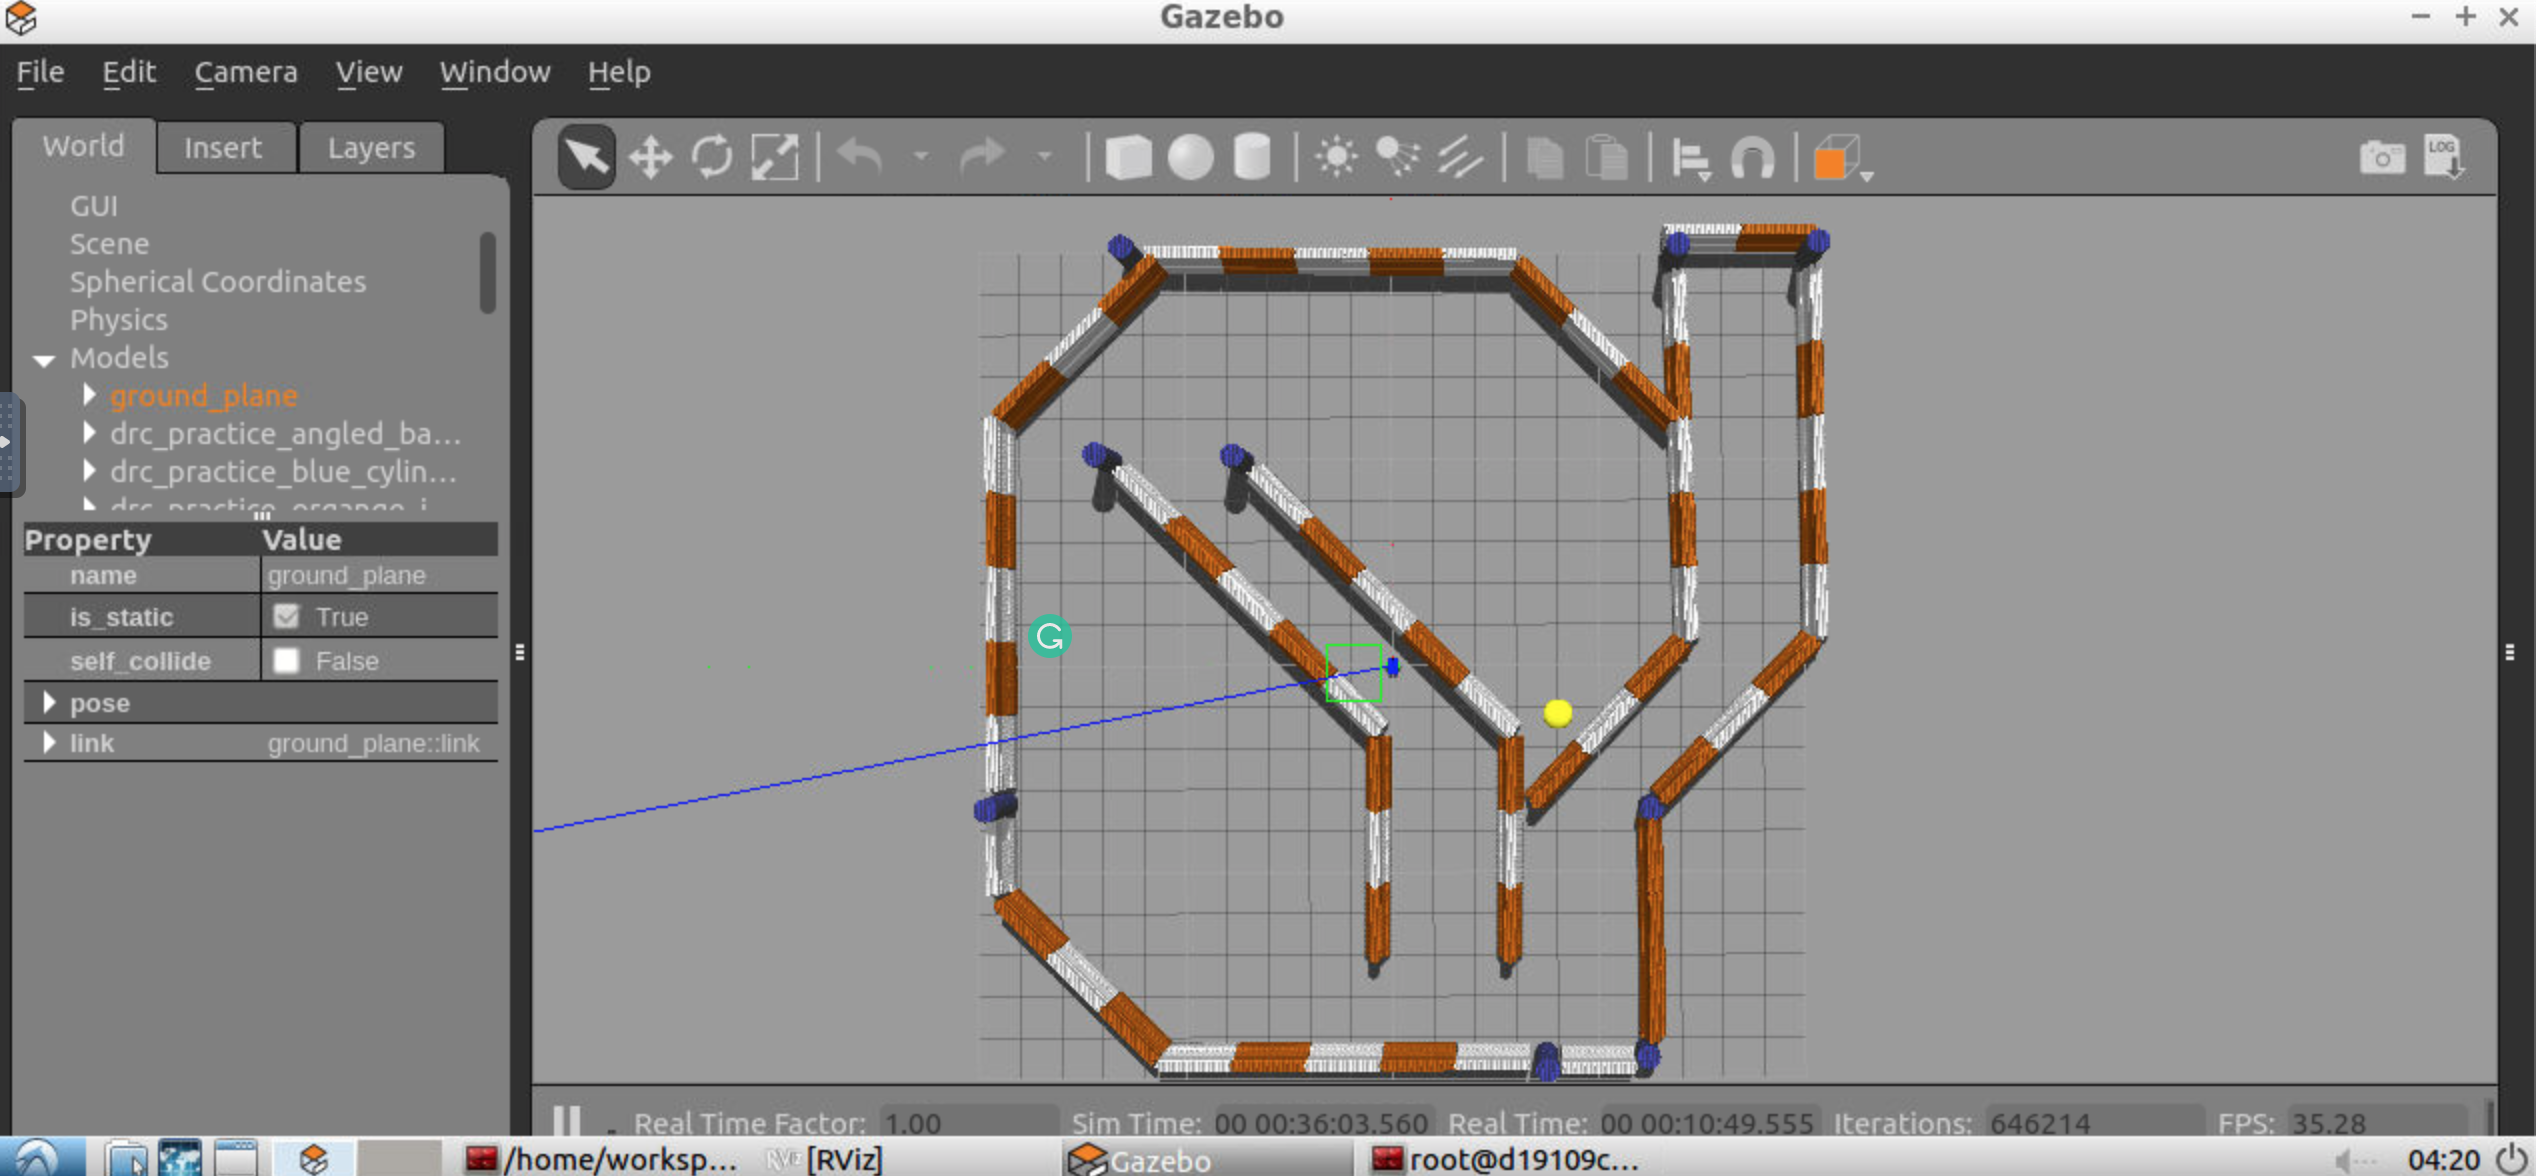
\includegraphics[width=\linewidth]{MapRobot.png}
      \caption{Robot Revolution.}
      \label{fig:robot1}
\end{figure}

\section{Background}
In the book Probabilistic Robotic (Thrun et al. 2005) described there are several approach to help robot perform localization problem from Extend Kalman filter to Marco, to Monte Carlo and finally Grid. In this project, Jackal race world is a local localization problem which has information robot's initial pose relate to static environment collecting sensory information using range finder sensors from environment.
.\cite{lamport1994latex}

\subsection{Kalman Filters}
 Kalman filters can take data with a lot of noisy or uncertainty in the measurements and provide very accurate estimate of the real value and can do it very fast don't need wait a lot of data to come. The Kalman Filter is applicable to problems with linear motion and measurement functions. This is limiting, as much of the real world is nonlinear.
 
\subsection{Particle Filters}
MCL can solve local and global localization problems represents non Gaussian distribution and can approximate any other practical important distribution not limited to linear model. 
\subsection{Comparison / Contrast}
MCL is easy to program compare to EKF. MCL uses particle to localize robot's pose and can approximate almost any state space distribution. MCL uses particles to localize a robot and can approximate almost any distribution. Each particle has a position and orientation by changing the number of particles control computational memory and resolution.
%example for inserting image
\begin{figure}[thpb]
      \centering
      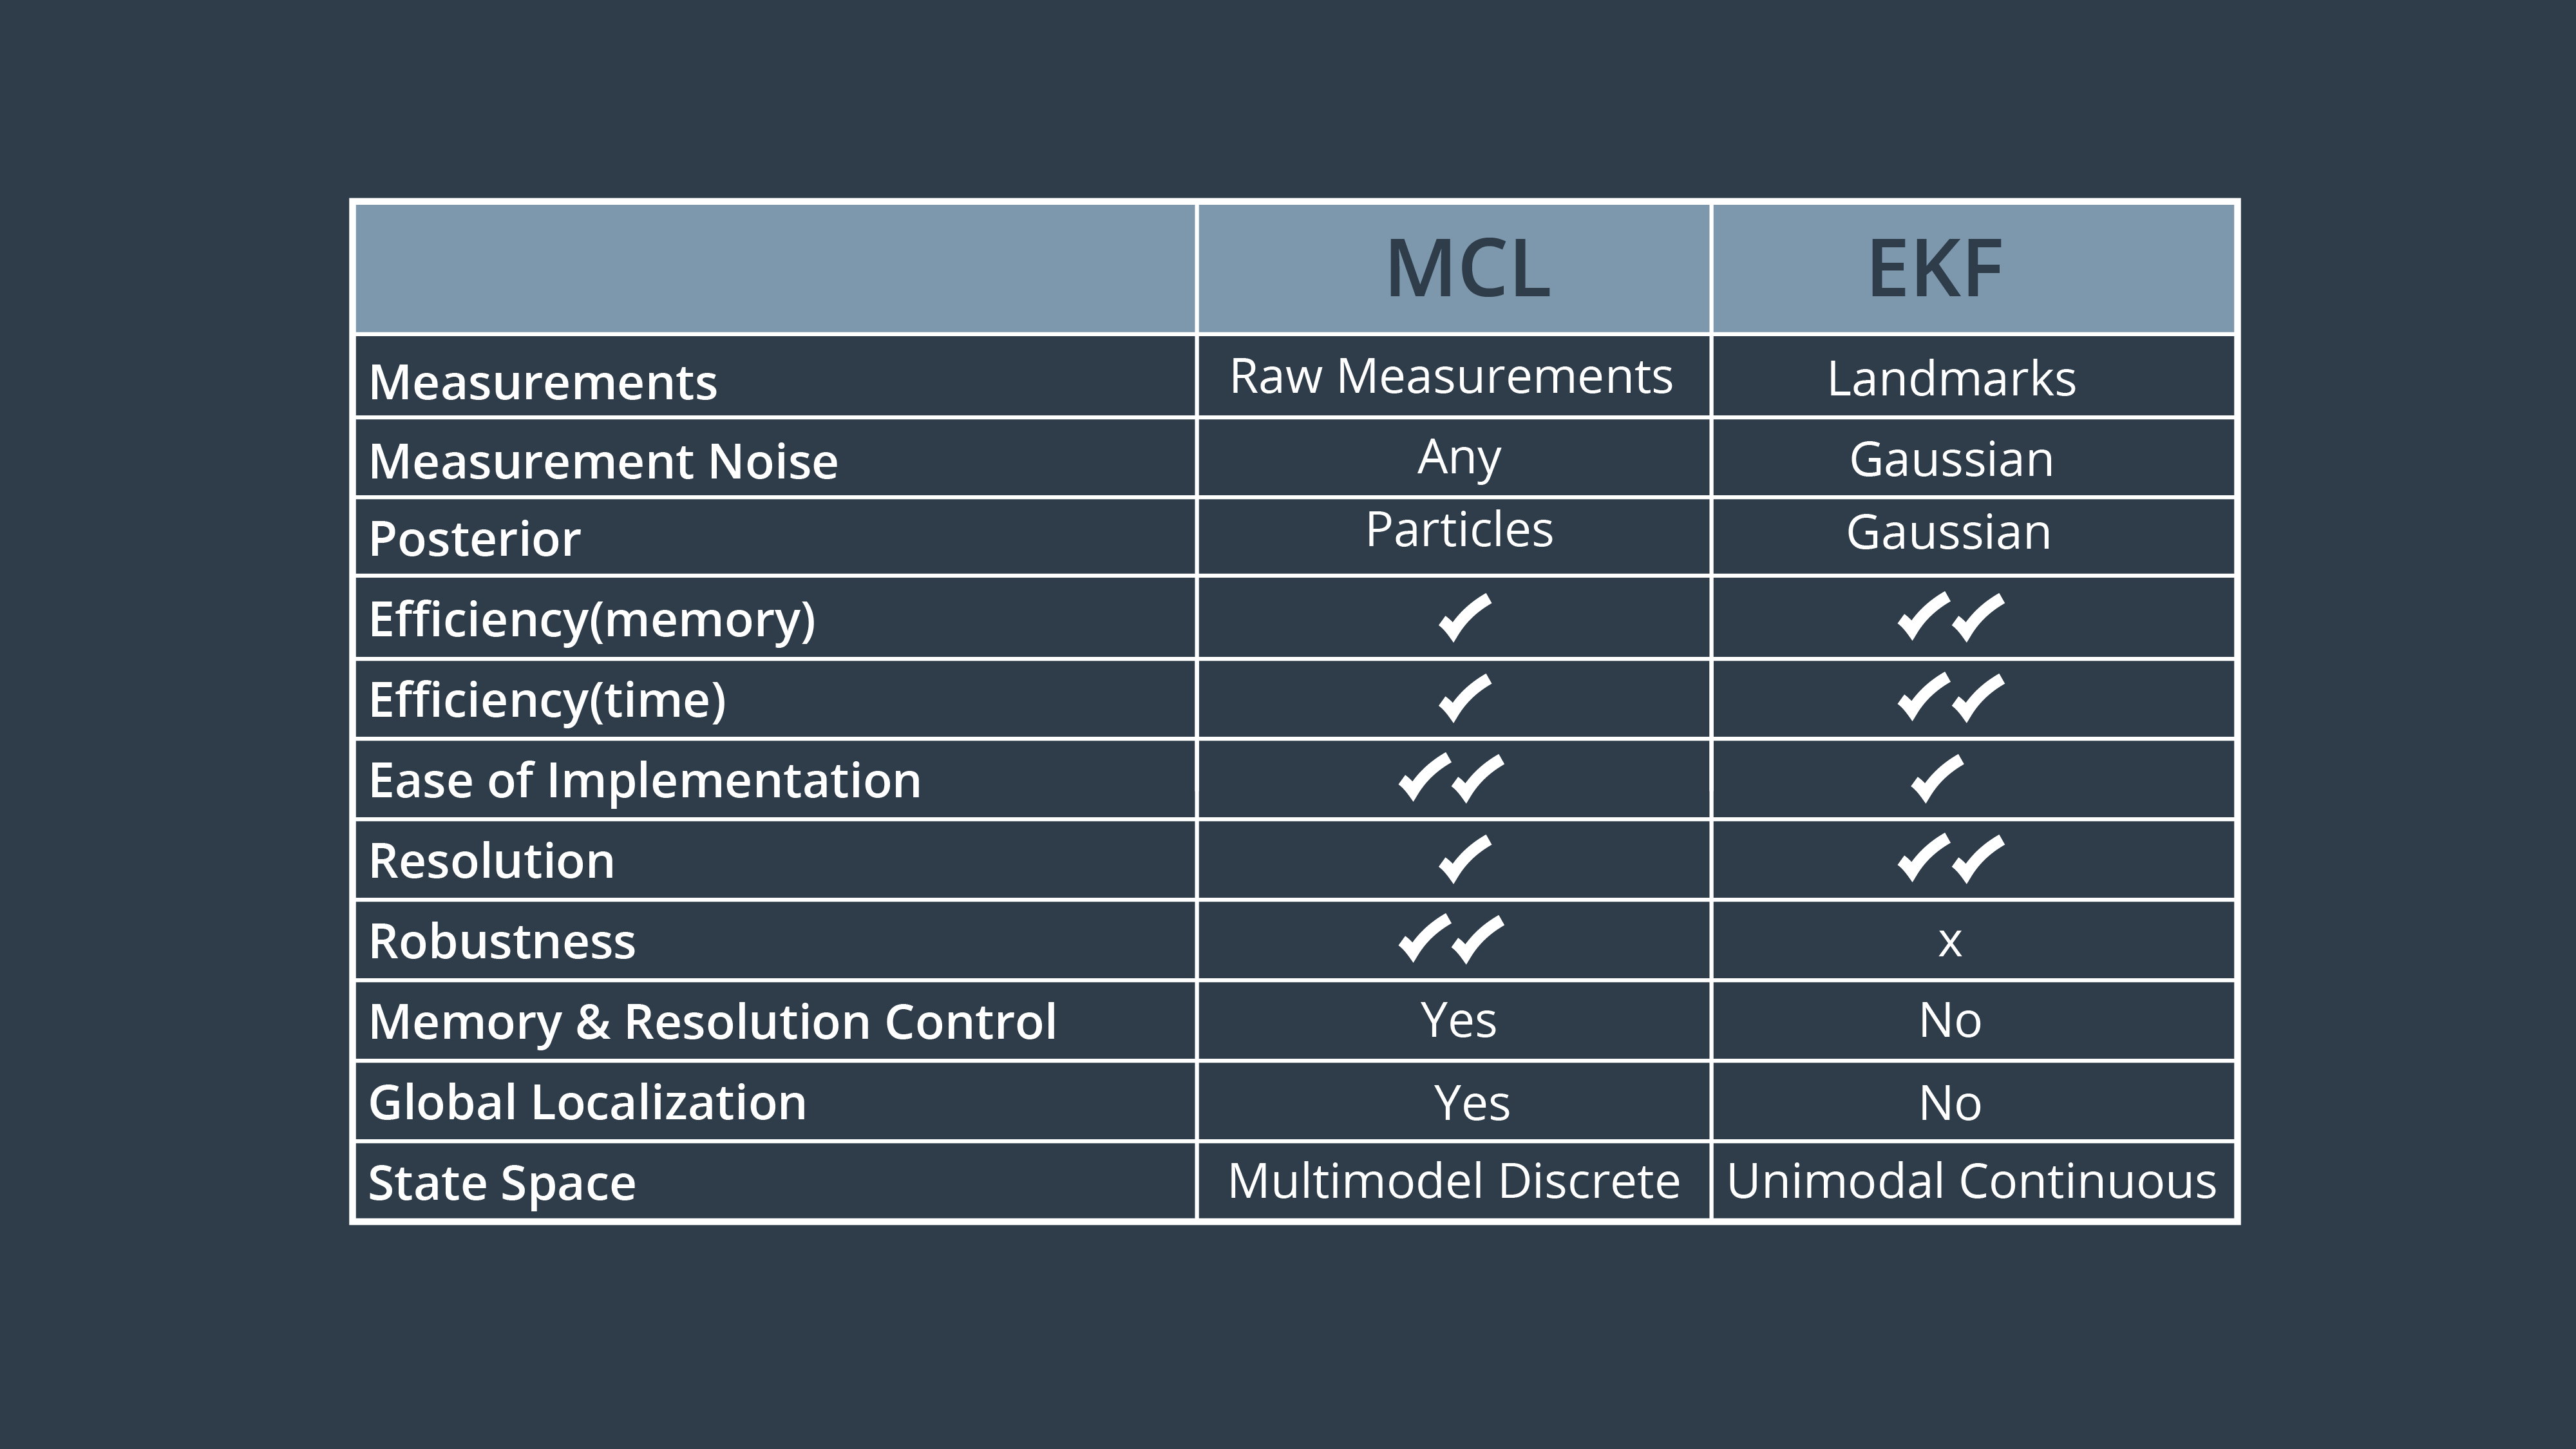
\includegraphics[width=\linewidth]{mclVsEKF.png}
      \caption{MCL VS EKF.}
      \label{fig:robot1}
\end{figure}
\section{Simulations}
 By utilize ROS packages to accurately localize a mobile robot inside a provided map in the Gazebo and RViz simulation environments. While Gazebo is a physics simulator, RViz can visualize any type of sensor data being published over a ROS topic like camera images, point clouds, Lidar data, etc. This data can be a live stream coming directly from the sensor or pre-recorded data stored as a bag file. RViz is one-stop tool to visualize all the three core aspects of a robot: Perception, Decision Making, and Actuation.  
 
 Over all ROS aspect:
\begin{itemize}
\item Building a mobile robot for simulated tasks.
\item Creating a ROS package that launches a custom robot model in a Gazebo world and utilizes packages like AMCL and the Navigation Stack.
\item Exploring, adding, and tuning specific parameters corresponding to each package to achieve the best possible localization results.
\end {itemize}

\subsection{Achievements}
You should describe what you achieved for localization in the project with the benchmark model and your own model. Includes charts and graphs show how parameters affect your performance. 

% Robot Models
\subsection{Benchmark Model: Udacity Bot}
\subsubsection{Model design}

%example for inserting image
\begin{figure}[thpb]
      \centering
      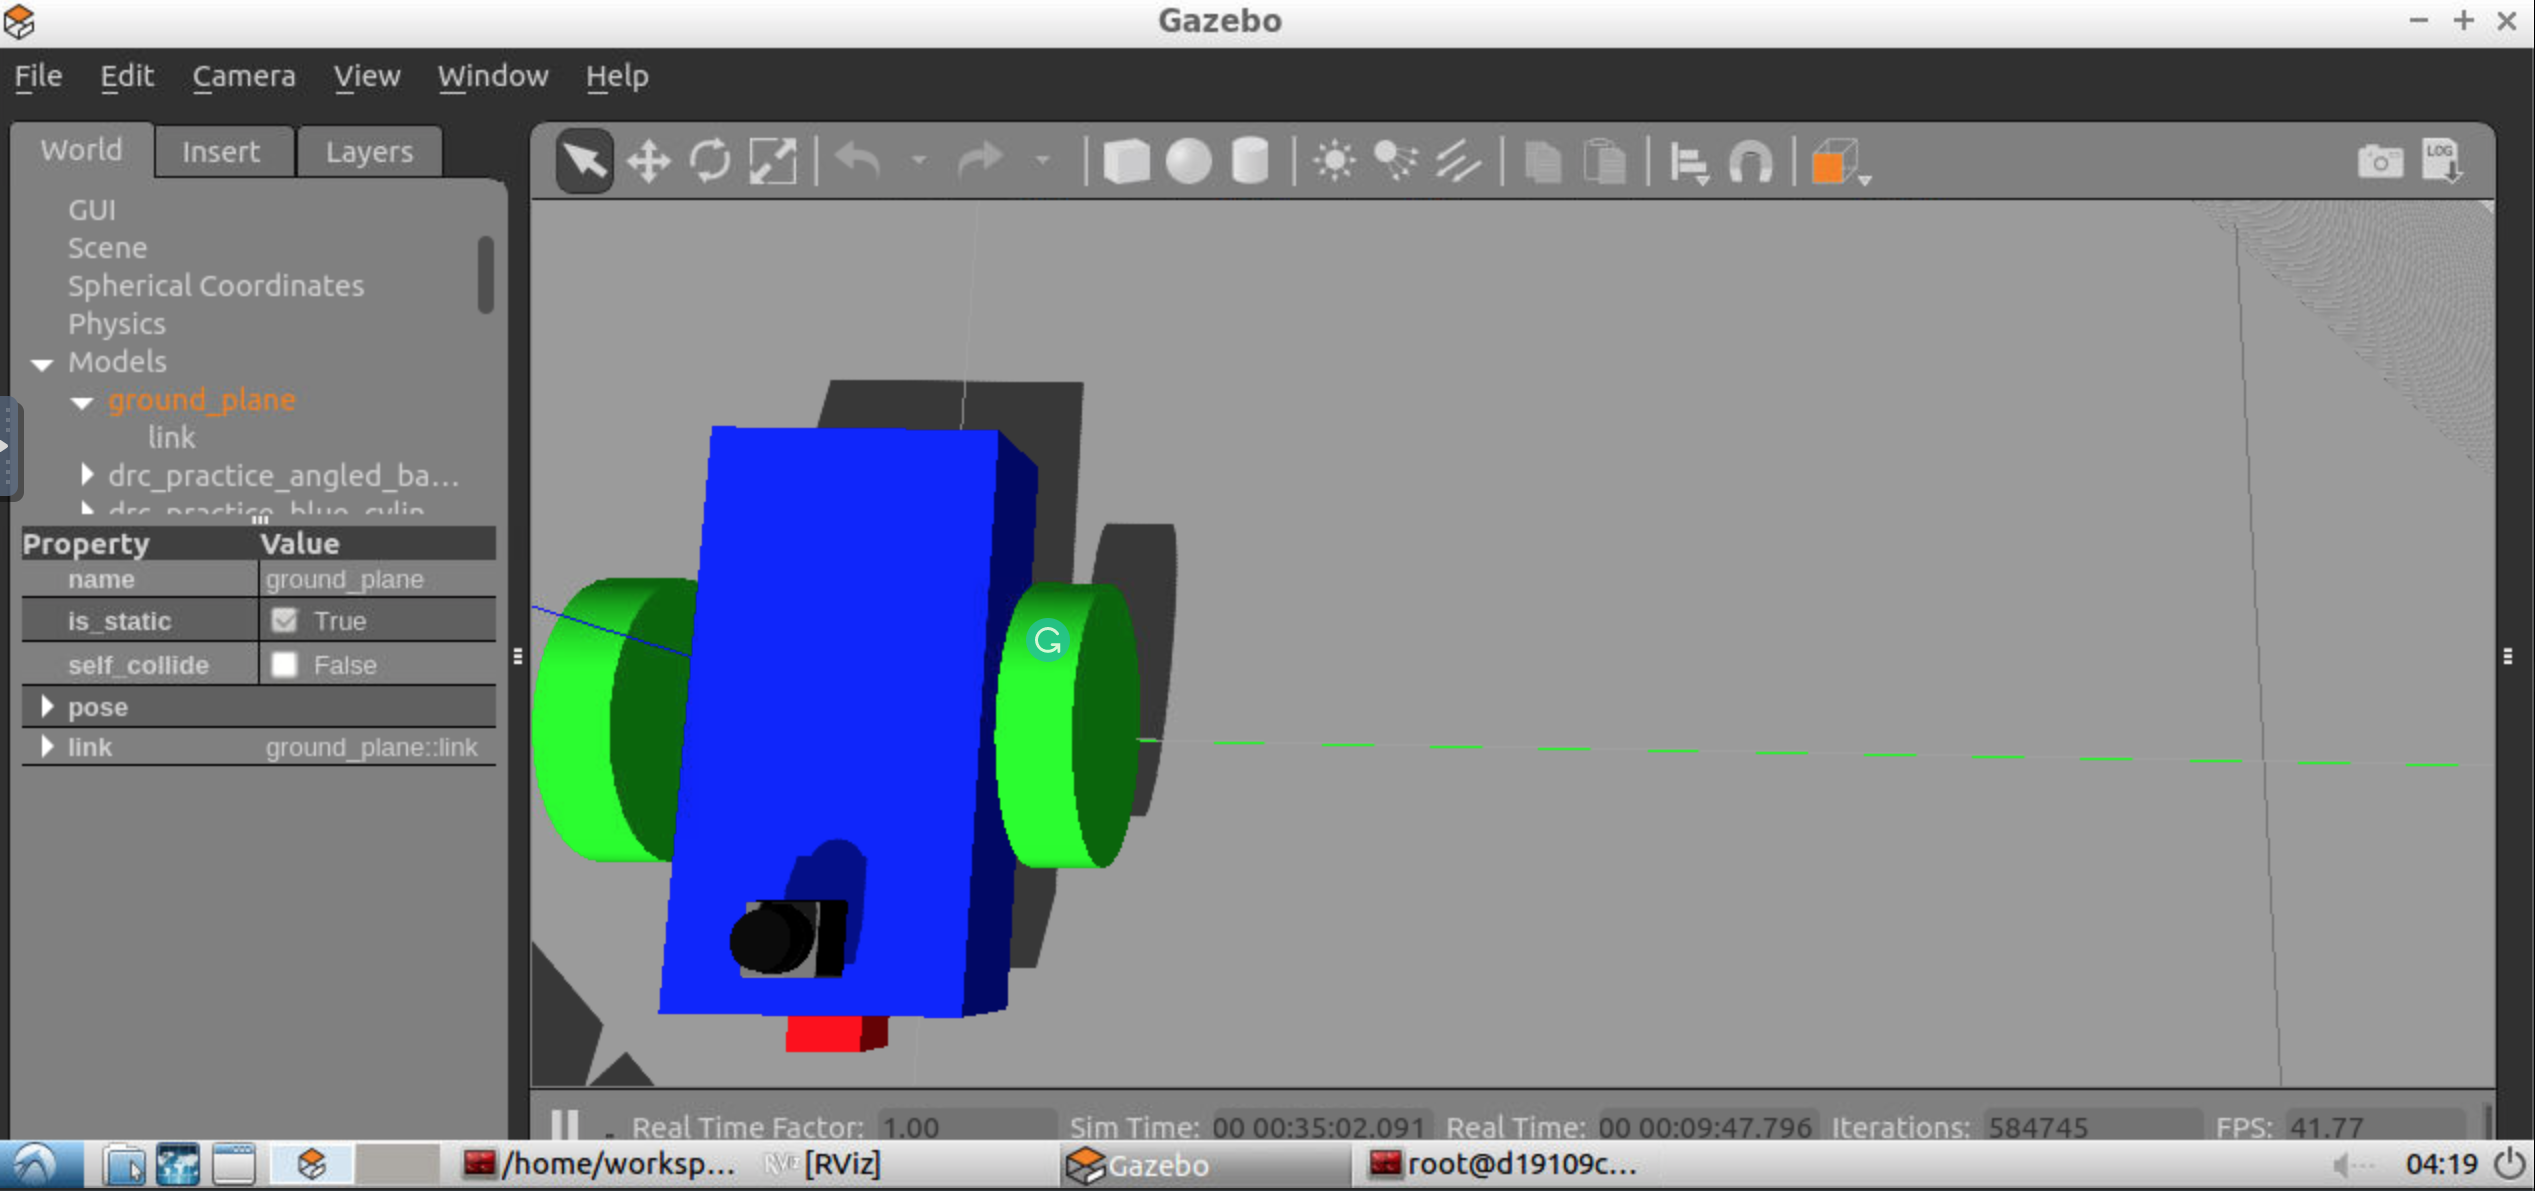
\includegraphics[width=\linewidth]{laserrangefinder.png}
      \caption{Robot model with a camera and laser rangefinder.}
      \label{fig:robot1}
\end{figure}
The Robot's design considerations should include: the size of the robot, the layout of sensors. This information can be shown in the form of a chart / table.
%example for building table
\begin{table}[h]
\caption{Table}
\label{table_example}
\begin{center}
\begin{tabular}{|c||c|}
\hline
One & Two\\
\hline
Three & Four\\
\hline
\end{tabular}
\end{center}
\end{table}
\subsubsection{Packages Used}
Udacity Bot package
\begin{itemize}
\item config
\item launch
\item maps
\item meshes
\item src
\item urdf
\item worlds
\item rviz
\end {itemize}
\subsubsection{Parameters}
Localization parameters in the AMCL node should be described, as well as move\_base parameters in the configuration file. You should be able to clearly demonstrate your understanding of the impact of these parameters.

\subsection{Personal Model}
% ditto
\subsubsection{Model design}
\subsubsection{Packages Used}
HsinBot package
\begin{itemize}
\item config
\item launch
\item maps
\item meshes
\item src
\item urdf
\item worlds
\item rviz
\end {itemize}
\subsubsection{Parameters}


\section{Results}
Present an unbiased view of your robot's performance and justify your stance with facts. Do the localization results look reasonable? What is the duration for the particle filters to converge? How long does it take for the robot to reach the goal? Does it follow a smooth path to the goal? Does it have unexpected behavior in the process? \\
For demonstrating your results, it is incredibly useful to have some watermarked charts, tables, and/or graphs for the reader to review. This makes ingesting the information quicker and easier.

\subsection{Localization Results}
\subsubsection{Benchmark}
%example for inserting image
\begin{figure}[thpb]
      \centering
      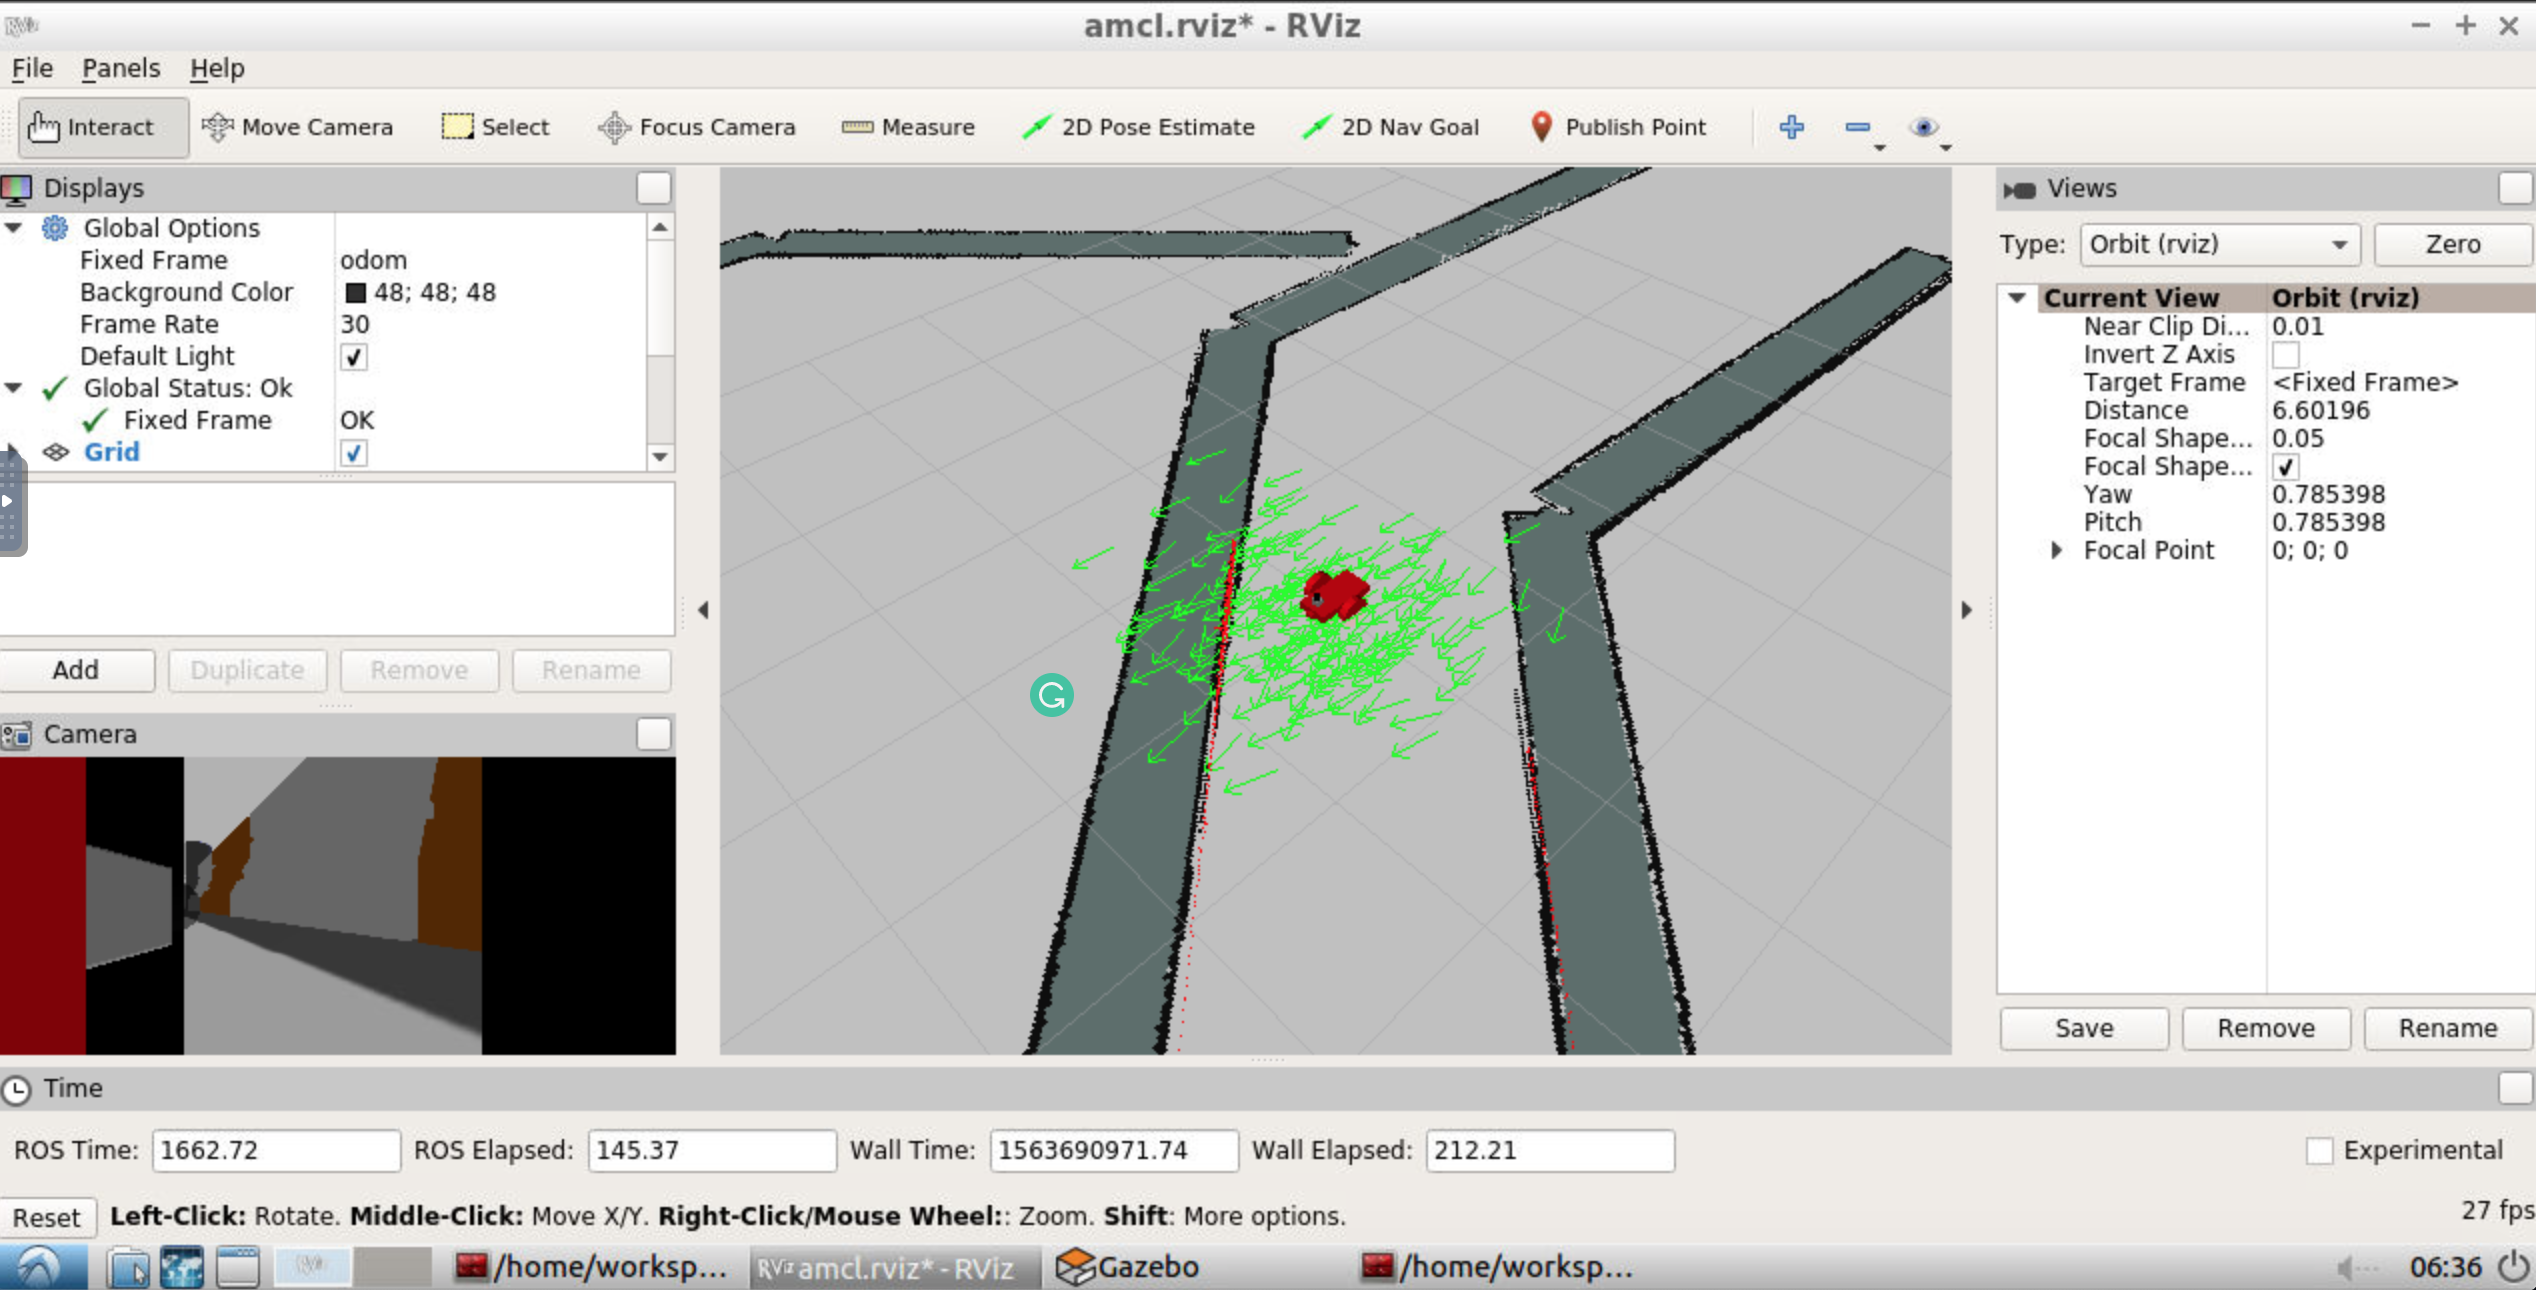
\includegraphics[width=\linewidth]{acml.png}
      \caption{Robot model with a camera and laser rangefinder.}
      \label{fig:robot1}
\end{figure}
%example for inserting image
\begin{figure}[thpb]
      \centering
      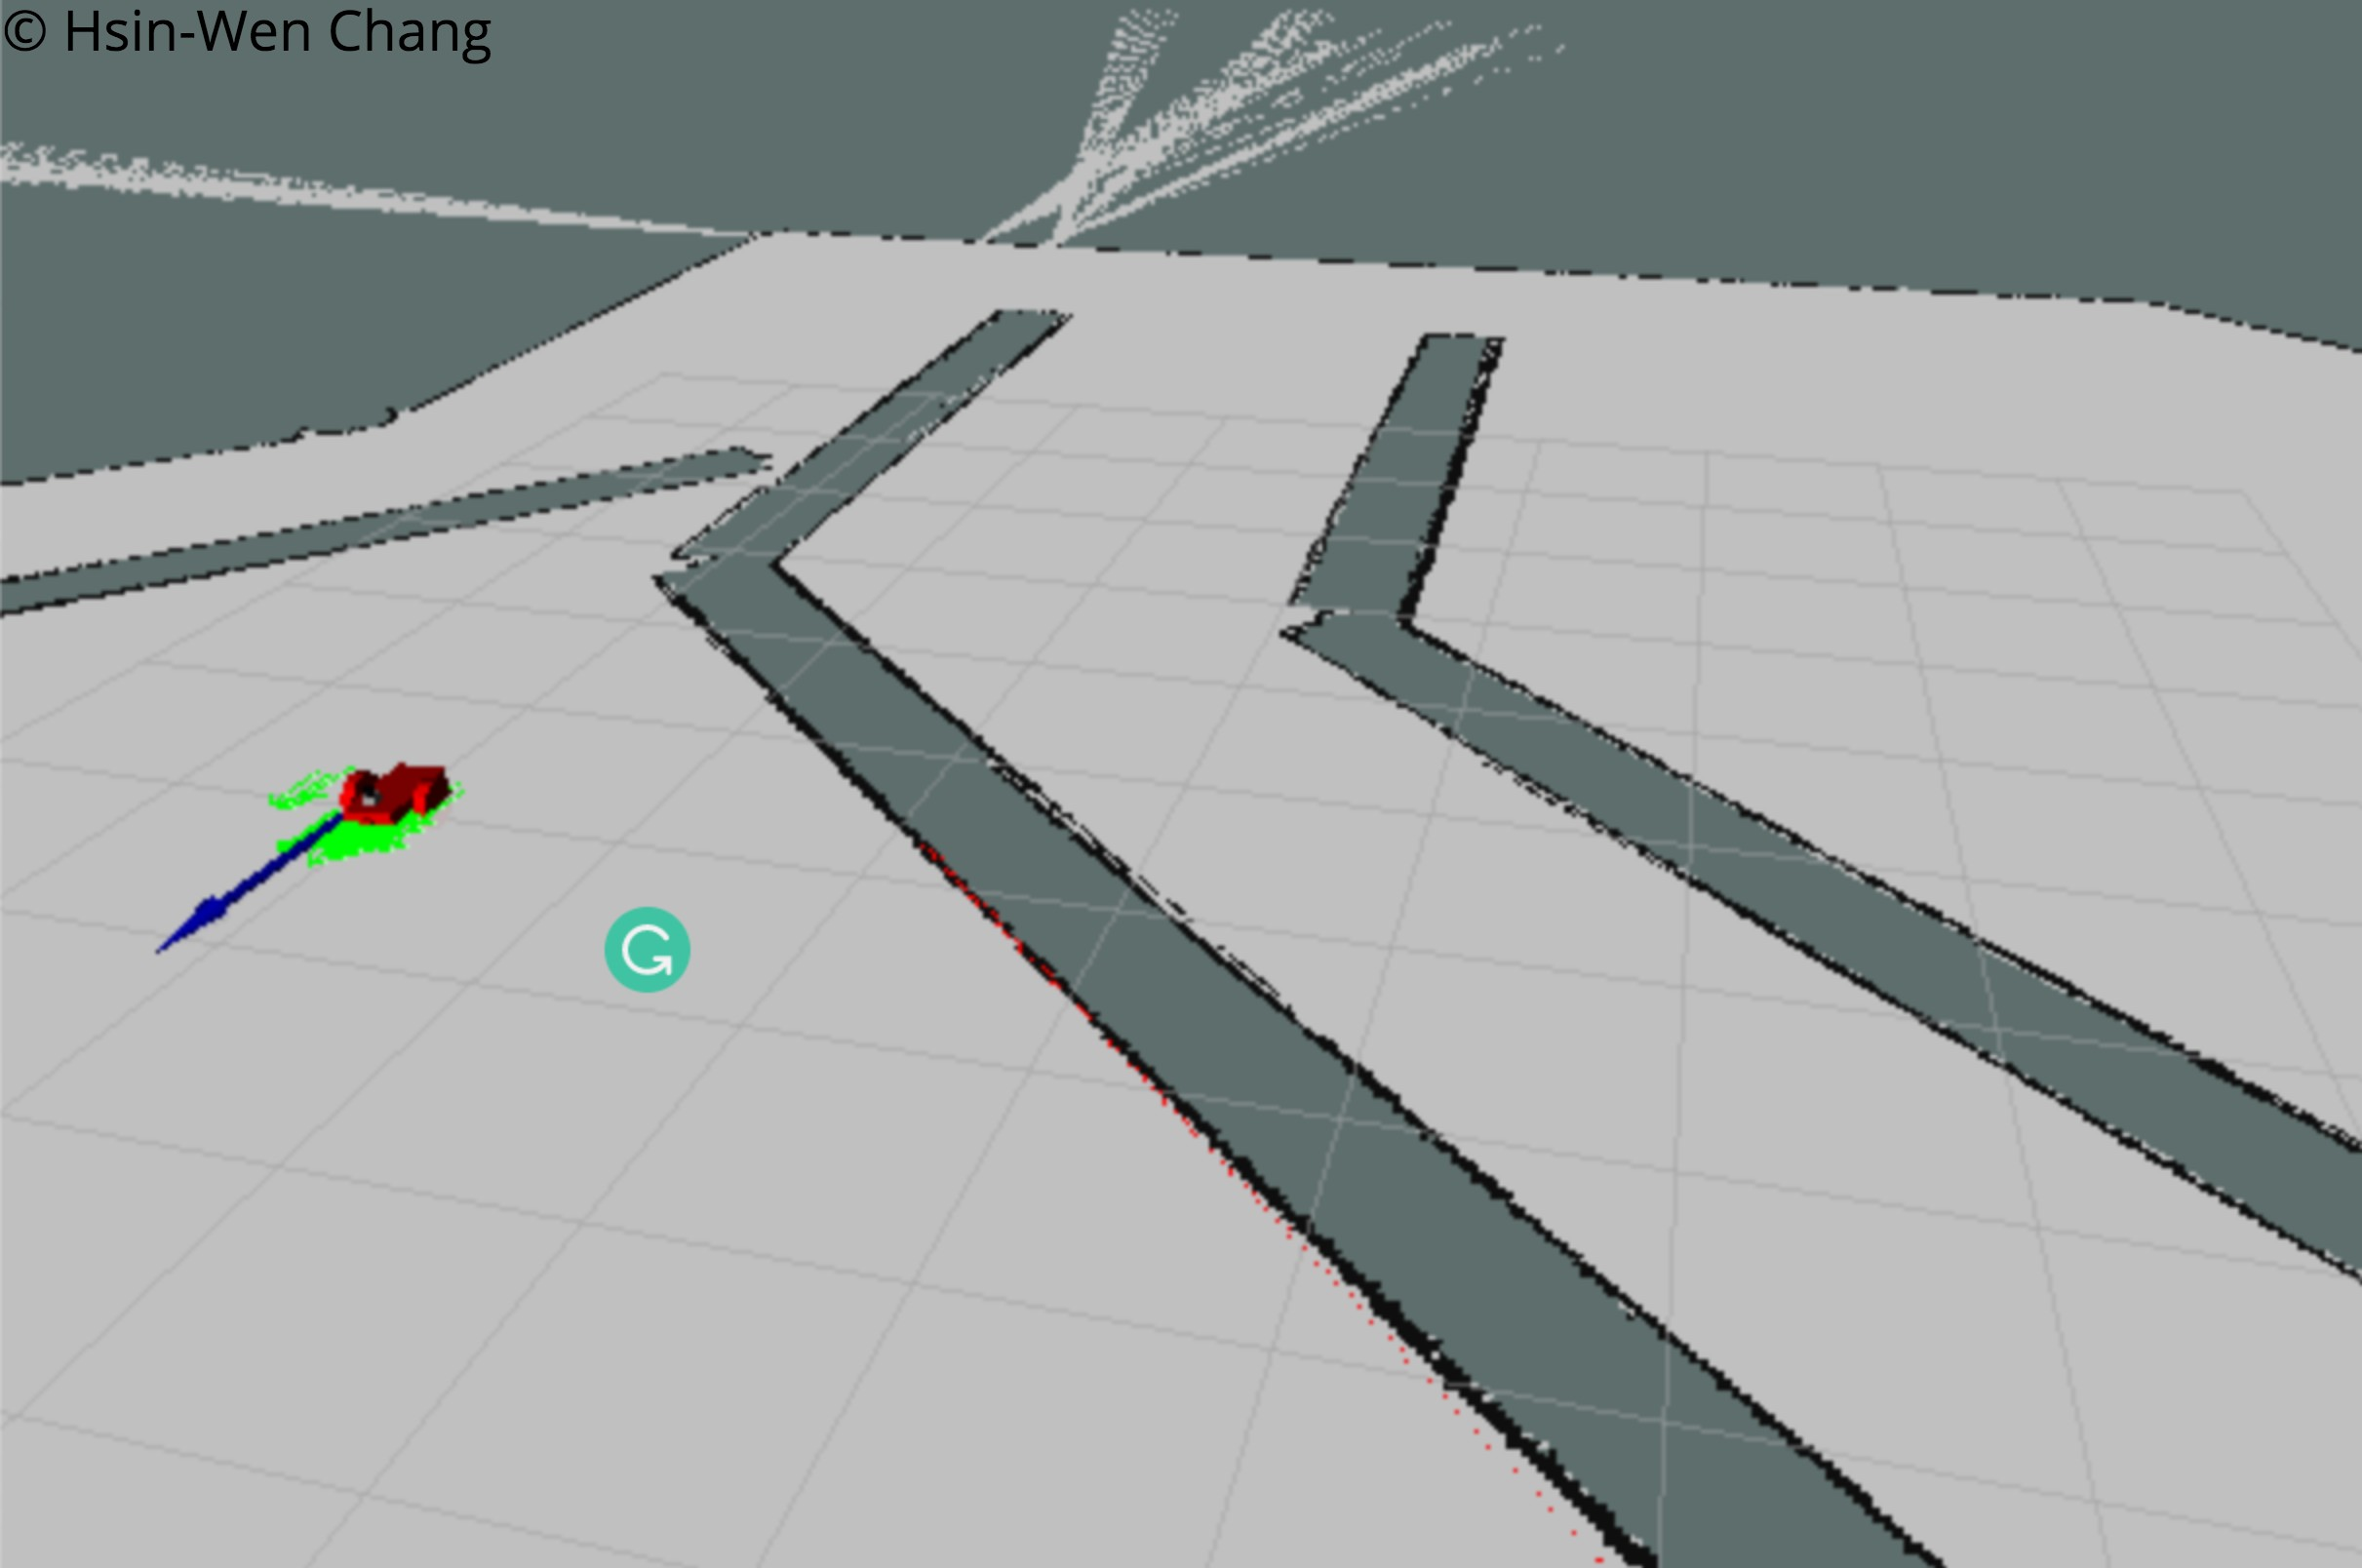
\includegraphics[width=\linewidth]{f2.png}
      \caption{Reaching the goal position.}
      \label{fig:robot1}
\end{figure}
\subsubsection{Student}

\subsection{Technical Comparison} % only facts
Discuss the difference of the layout, parameters, performance etc. between the benchmark robot and your robot. It is acceptable for your custom robot to perform worse than the provided robot. The focus is on learning and understanding, not performance. 

\section{Discussion}
This is the only section of the report where you may include your opinion. However, make sure your opinion is based on facts. If your robot performed poorly, make mention of what may be the underlying issues. If the robot runs well, which aspects contribute to that? Again, avoid writing in the first person (i.e. Do not use words like "I" or "me"). If you really find yourself struggling to avoid the word "I" or "me"; sometimes, this can be avoid with the use of the word “one”. As an example: instead of : "I think the robot cannot localize itself because the sensor does not provide enough information for localization" try: "one may believe the localization performance is poor because the sensor layout is not able to provide enough information for localization". They say the same thing, but the second avoids the first person. 

\subsection{Topics}
\begin{itemize}
\item Which robot performed better?
\item Why it performed better? (opinion)
\item How would you approach the 'Kidnapped Robot' problem?
\item What types of scenario could localization be performed?
\item Where would you use MCL/AMCL in an industry domain?
\end {itemize}

\section{Conclusion / Future work}
This section is intended to summarize your report. Your summary should include a recap of the results, did this project achieve what you attempted, how would you deploy it on hardware and how could this project be applied to commercial products? 
For Future Work, address areas of work that you may not have addressed in your report as possible next steps. This could be due to time constraints, lack of currently developed methods / technology, and areas of application outside of your current implementation. Again, avoid the use of the first-person.

\subsection{Modifications for Improvement}
Examples:
\begin{itemize}
\item Base Dimension
\item Sensor Location
\item Sensor Layout
\item Sensor Amount
\end{itemize}

\subsection{Hardware Deployment}
\begin{enumerate}
\item What would need to be done?
\item Computation time/resource considerations?
\end{enumerate}



\bibliography{bib}
\bibliographystyle{ieeetr}

\end{document}